%evaluation.tex

\chapter{Evaluation}
\label{chapter:eva}
\todo{Kapitel Evaluation schreiben}

Was kann ich mit meinem Modell?

Simulation von Peaks die ideal-gaußförmig sind oder tailing aufweisen

Grenzen des Modells:
Minimalbreite kann nicht unterschritten werden


Formel zur Umrechnung von Peakdaten in Parameter, oder falls das nicht drin ist, zumindest Zusammenhänge, dazu zb Plots von drei festen Parametern
Evtl Tabelle mit exemplarischen Daten?
Sinnvolle Parameterbereiche

3a modell liefert tailing, welches bei 3b nicht gefunden wurde (vielleicht einfach nur die falschen parameter ausprobiert?)

\section{Relevanter Parameterbereich / relevate Peaks}

\todo{Strukur: erst komplett 2p dann 3s, wegen referenz auf schiefe bei 2p in den params für 3s}

\subsection{2-Parameter Modell}


\subsection{3-Zustände Modell}
\todo{Wo erwähnen, dass nach 240 sec Schluss ist?}


Die wenigen Peaks, die beim 2-Parameter Modell Schiefe aufweisen dienen als Grundlage für eine sinnvolle Parametereinschränkung für pml und pll. Dabei war zu beobachten, dass die Teilchen nur selten in den stationären Zustand eintreten, dafür aber sehr lange dort verweilen. Um diesen Effekt nachzuahmen, muss pml dementsprechend sehr klein im Vergleich zu pma und pmm sein. pll muss dafür sehr groß sein, deutlich größer als paa

In der experimentellen Phase der Arbeit wurden zunächst im gesamten Parameterraum $[0;1]^3$ einige Simulationen durchgeführt, um herauszufinden, in welchen Bereichen sich Peaks ergeben. 
Durch die Beschränkung des Spektrums auf $240$ Sekunden scheiden schon viele Parameterkombinationen aus, welche spätere Peaks erzeugen würden. Das betrifft insbesondere diejenigen Kombinationen, die eine geringe Wahrscheinlichkeit haben, mobil zu bleiben oder zu werden, dafür aber mit einer sehr hohen Wahrscheinlichkeit stationär werden oder bleiben. 
% Für die Schiefe soll es zunächst keine Beschränkungen geben, TODO (gibt es ne sinnvolle Obergrenze, Optik mit Werten vergleichen)
Typischerweise sind Peaks zu Beginn des Spektrums eher schmal, spätere Peaks können breiter werden. Generell lässt sich sagen, dass der IQR eines Peaks geringer sein sollte, als sein Maximalzeitpunkt. Darüber hinaus wurde eine maximale Peakbreite von 10+0.2*maxzeitpunkt TODO festgelegt. Peaks mit höherem IQR sind in einem Spektrum kaum noch als Peaks zu erkennen.
Sehr breite Peaks sind auch nur dann als Peak zu erkennen, wenn sie sehr schief sind.
Für die Schiefe gilt, dass ein Tailing ab einem IQK von 0.2 gut zu erkennen ist. Werte bis 0.4 treten meist bei schiefen Peaks auf, die auch optisch einem realistischen Peak ähneln. Darüber hinaus haben die Peaks oft ein sehr langes Tailing, welches teilweise auch über die Maximalzeit hinausragt. Dieses ist jedoch auf einem so niedrigen Niveau, dass es in einem Spektrum mit Rauschen wahrscheinlich unter gehen würde.
\todo{bewertende aussagen weglassen, habe ja keine vergleichsdaten}
Dadurch ergeben sich folgende Einschränkungen für die verschiedenen Parameter:
\begin{itemize}
 \item $p_{mm}$: keine generellen Einschränkungen, es wurden für Werte im Intervall $[0,005; 0,99]$ Peaks gefunden. Bei noch kleineren Werten TODO bei größeren Werten TODO
 \item $p_{ml}$: sinnvolle Werte liegen im Bereich $[0,00001; 0,001]$. Bei kleineren Werten ergeben sich auch Peaks, die jedoch kein oder fast kein Tailing mehr aufweisen, sodass auch auf das zwei-Parameter-Modell zurückgegriffen werden kann. Bei größeren Werten verweilen die Teilchen so lange im gelösten Zustand, dass die Peaks extrem breit werden, insbesondere, wenn der Parameter $p_{ll}$ auch sehr groß gewählt wurde.
 \item $p_{aa}$: für diesen Parameter wurde der das Intervall auf $[0.997, 0.9996]$ beschränkt. Kleinere Werte sorgen für extrem frühe Peaks. Diese könnten zwar berücksichtigt werden, unterscheiden sich jedoch kaum voneinander. Bei größeren Werten werden die Peaks meist zu breit und zu spät. 
 \item $p_{ll}$: sinnvolle Werte liegen im Bereich $[0,9999; 0,999995]$. Kleinere Werte TODO Bei größeren Werten werden die Teilchen so lange im stationären Zustand gehalten, dass die Peaks meist über das Maximum von 240 Sekunden hinausragen oder zu breit werden. Dies gilt insbesondere, wenn für $p_{ml}$ ebenfalls ein großer Wert gewählt wurde. Im oberen Bereich des Intervalls (>0.999995 erzeugen werden hier Peaks erzeugt, die eine sehr große Schiefe aufweisen, wo der Tail jedoch (wahrscheinlich) im Rauschen verschwindet. Mit den aktuellen Maßen lässt sich das kaum zeigen, wird jedoch beim Blick auf einen geplotteten Peak sofort klar.
\end{itemize}

In allen Fällen gilt jedoch, dass auch jeweils die Kombination der Parameter berücksichtigt werden muss, insbesondere, wenn ein Parameter am Rand des jeweils angegebenen Intervalls liegt, kommt es häufig vor, dass er nur in einigen wenigen Kombinationen für realistische Peaks sorgt.
Beispiele: TODO: ein paar Kombis nennen, die grenzwertig, bzw drüber hinaus sind.



\section{Einfluss der verschiedenen Parameter auf Peaks}

\subsection{2-Parameter Modell} 

Sowohl Zeitpunkt als auch Breite der Peaks hängen von ps und pm ab.
Nur in einem sehr kleinen Bereich, bei dem die Peaks ihren Maximalzeitpunkt bei etwa TODO haben, tritt überhaupt Schiefe auf. 


\subsection{3-Zustände Modell}

In den meisten Fällen kann ein deutlicher Zusammenhang zwischen den Parametern und Peakdaten beobachtet werden, diese seien im Folgenden aufgeführt.
Für den Maximalzeitpunkt des Peaks sowie seine Breite gilt, dass beide größer werden, wenn die Parameter $p_{ml}$, $p_{aa}$ und $p_{ll}$ größer werden oder $p_{mm}$ kleiner wird. 
Die Schiefe steigt mit steigendem $p_{ll}$ und fallendem $p_{aa}$. Für $p_{ml} \text{ und } p_{mm}$ ist zu beobachten, dass bei größer werdenden Parametern die Schiefe zunächst auch ansteigt, ab einem gewissen Wert jedoch sinkt. 
Da bei einem Wert für $p_{ml}$ effektiv das zwei-Parameter-Modell zum Einsatz kommt, ist hier fast nie Schiefe zu beobachten, außerdem hat der Parameter $p_{ll}$ keinen Einfluss. 


$p_{aa}$ hat einen stärkeren Einfluss auf den Zeitpunkt als $p_{ll}$ und $p_{ml}$. Dieser wird noch stärker, wenn $p_{mm}$ klein ist

$p_{mm}$ hat einen großen Einfluss auf den Zeitpunkt und nur einen minimalen Einfluss auf die Breite.

$p_{ml}$ und $p_{ll}$ haben zunächst beide einen proportionalen Einfluss auf die Schiefe. Erst, wenn beide sehr groß sind, sinkt die Schiefe wieder (und die Breite steigt extrem an) Das ist wohl dadurch zu erklären, dass sich nicht mehr genügend Teilchen im mobil-adsorbierten System befinden, wodurch ein normaler Peak entstehen kann. Statt dass die Lösung Schiefe an diesem einfachen Peak verursacht, sorgt sie nunmehr für Breite

Tailing/Schiefe entsteht immer da, wo nur wenige Teilchen langsamer sind, als die große Masse. Sind viele Teilchen lange stationär, werden die Peaks statt dessen breit. Der Maximalzeitpunkt ist hauptsächlich durch die Durchschnittsgeschwindigkeit der Teilchen bestimmt, sind sie hauptsächlich mobil, entstehen frühe Peaks, sind sie oft und lange stationär, wandern die Peaks nach hinten.

\begin{figure}[H]
\begin{subfigure}[t]{0.5\textwidth}
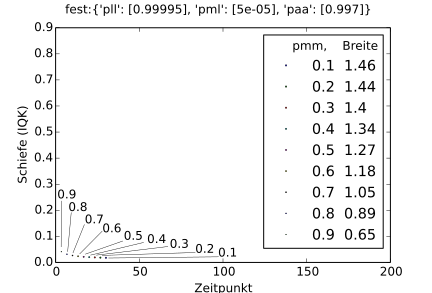
\includegraphics[width=\textwidth]{bilder/3fest_p_000005_0997_099995.pdf}
\caption{$p_{mm}$ und $p_{ml}$ groß}
\end{subfigure}
\begin{subfigure}[t]{0.5\textwidth}
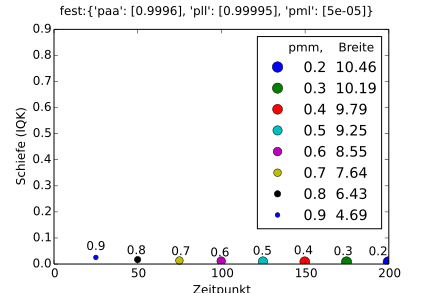
\includegraphics[width=\textwidth]{bilder/3fest_p_000005_09996_099995.pdf}
\caption{$p_{mm}$ groß und $p_{ml}$ klein}
\end{subfigure}
\caption{Der Einfluss von $p_{mm}$ auf die Breite abhängig von $p_{mm}$}
\label{einfluss_pmm_1}
\end{figure}

Wie in Abbildung \ref{einfluss_pmm_1} zu sehen, ist der Einfluss von $p_{mm}$ auf den Zeitpunkt von $p_{aa}$ abhängig: Je größer $p_{aa}$ ist, desto stärker wird der Zeitpunkt von $p_{mm}$ beeinflusst. Wenn $p_{mm}$ und $p_{aa}$ klein sind, entstehen nur Peaks zu Beginn des Spektrums, unabhängig von $p_{ml}$ oder pll.
Der Einfluss von $p_{mm}$ auf die Breite ist gering, bei größerem PAA steigt dieser Einfluss etwas, wie ebenfalls in Abbildung \ref{einfluss_pmm_1} zu erkennen ist. Dieser Einfluss hängt damit zusammen, dass sich in diesem Fall auch der Maximalzeitpunkt nach hinten verschiebt und spätere Peaks generell breiter sind, als frühe Peaks.
%, was aber wahrscheinlich auch mit dem in diesem Fall ansteigenden Zeitpunkt zu tun hat (Peaks haben dem maxzeitpunkt auf dem gesamten Spektrum und werden mit zunehmender Zeit auch breiter)

% \begin{figure}[H]
% \begin{subfigure}[t]{0.5\textwidth}
% \includegraphics[width=\textwidth]{bilder/}
% \caption{$p_{aa}$ groß und $p_{ml}$ groß}
% \end{subfigure}
% \begin{subfigure}[t]{0.5\textwidth}
% \includegraphics[width=\textwidth]{bilder/}
% \caption{$p_{aa}$ groß und $p_{ml}$ klein}
% \end{subfigure}
% \vspace*{7mm}
% \begin{subfigure}[b]{0.5\textwidth}
% \includegraphics[width=\textwidth]{bilder/}
% \caption{$p_{aa}$ klein und $p_{ml}$ groß}
% \end{subfigure}
% \begin{subfigure}[b]{0.5\textwidth}
% \includegraphics[width=\textwidth]{bilder/}
% \caption{$p_{aa}$ klein und $p_{ml}$ klein}
% \end{subfigure}
% \caption{Der Einfluss von $p_{mm}$ auf die Schiefe abhängig von $p_{aa}$, $p_{ml}$ und $p_{ll}$}
% \label{einfluss_pmm_2}
% \end{figure}


TODO: Noch mal den kleinen Bereich untersuchen, wo die Schiefe negativ beeinflusst wird. Das ist ein Bereich, in dem die Peaks zwar sehr früh, aber dafür fast zu breit sind. Vielleicht hängt das damit zusammen? siehe: $p_{mm}$0.001 0.998 0.99999
Ansonsten steigt die Schiefe mit steigendem pmm. Dieser Einfluss hängt noch von $p_{aa}$ab, bei kleinem $p_{aa}$hat $p_{mm}$einen größeren Einfluss auf die Schiefe. Hängt aber auch von pml/pll ab! 
Einfluss am nur vorhanden bei mittlerem $p_{ml}$ (0,0001, 0,0005). Ist $p_{ml}$ zu klein, hat die Lösung fast keinen Einfluss, ist $p_{ml}$zu groß, werden die Peaks wieder nur breit, aber nicht so schief. Gleiches gilt für $p_{ll}$ (pmm beeinflusst Schiefe bei $p_{ll}$ von 0,99995-0,99999).
Wahrscheinlich, weil dadurch, dass $p_{aa}$ klein ist, der Einfluss von $p_{ml}$ und $p_{ll}$ größer wird. $p_{ml}$ und $p_{ll}$ verursachen ja gemeinsam das Tailing, dieser Tailingeffekt kann sich aber nur bei großem $p_{mm}$ durchsetzen, da die Teilchen, die nicht in den gelösten Zustand kommen, sich recht schnell fortbewegen (daher auch besonders bei kleinem $p_{aa}$ zu beobachten) und dadurch nur wenige Teilchen langsamer sind und dadurch den Tail verursachen. Ist kleiner, lösen sich die Teilchen häufiger und statt der schiefen entstehen breite Peaks
Ist $p_{aa}$ zu klein und $p_{ll}$ zu groß entstehen peaks, die zwar einen extrem großen iqk haben. Allerdings ist der Tail so flach, dass er in einem Gesamtchomatogramm wohl eher im Rauschen untergehen würde.


\begin{figure}
\begin{subfigure}[t]{0.5\textwidth}
\includegraphics[width=\textwidth]{bilder/pml/pml_01_p_0997_099999}
\caption{$p_{ll}$ sehr groß}
\end{subfigure}
\begin{subfigure}[t]{0.5\textwidth}
\includegraphics[width=\textwidth]{bilder/pml/pml_05_p_09994_0999995}
\caption{$p_{ll}$ groß}
\end{subfigure}
\vspace*{7mm}
\begin{subfigure}[b]{0.5\textwidth}
\includegraphics[width=\textwidth]{bilder/pml/pml_05_p_0998_099995}
\caption{$p_{ll}$ klein}
\end{subfigure}
\begin{subfigure}[b]{0.5\textwidth}
\includegraphics[width=\textwidth]{bilder/pml/pml_09_p_0999_09999}
\caption{$p_{ll}$ sehr klein}
\end{subfigure}
\caption{Der Einfluss von $p_{ml}$ auf die Schiefe und Breite abhängig von $p_{ll}$}
\label{einfluss_pml_1}
\end{figure}

Der Einfluss von $p_{ml}$ auf die Peakdaten ist in Abbildung \ref{einfluss_pml_1} gezeigt. Der Zeitpunkt ist nur minimal von pml abhängig. Die Punkte liegen fast auf einer Geraden oder nur leicht schrägen Linie nach oben. Allenfalls sehr große Werte für pml sorgen für einen deutlich erkennbaren höheren Zeitpunkt, dann aber auch für deutlich mehr Breite und weniger Schiefe.
Auf die Schiefe ist der Einfluss von pml sehr groß, wenn auch $p_{ll}$ groß ist. Gleiches gilt für die Breite, auch diese wird nur deutlich von pml beeinflusst, wenn auch pll groß ist. 

\begin{figure}
\begin{subfigure}[t]{0.5\textwidth}
\includegraphics[width=\textwidth]{bilder/pml/pml_09_p_0997_099995}
\caption{$p_{mm}$ groß, paa klein}
\end{subfigure}
\begin{subfigure}[t]{0.5\textwidth}
\includegraphics[width=\textwidth]{bilder/pml/pml_09_p_0997_099995}
\caption{$p_{mm}$ groß, paa groß}
\end{subfigure}
\vspace*{7mm}
\begin{subfigure}[b]{0.5\textwidth}
\includegraphics[width=\textwidth]{bilder/pml/pml_01_p_0997_099995}
\caption{$p_{mm}$ klein, paa klein}
\end{subfigure}
\begin{subfigure}[b]{0.5\textwidth}
\includegraphics[width=\textwidth]{bilder/pml/pml_01_p_09994_099995}
\caption{$p_{mm}$ klein, paa groß}
\end{subfigure}
\caption{Der Einfluss von $p_{ml}$ auf die Schiefe und Breite abhängig von $p_{mm}$ und paa}
\label{einfluss_pml_2}
\end{figure}

Wie in Abbildung \ref{einfluss_pml_2} gezeigt, spielen auch pmm und paa für den Einfluss von pml nur eine  Rolle. Ist paa klein, wird der Einfluss von pml auf Schiefe und Breite größer, ist pmm klein, wird der Einfluss auch kleiner.


%, wie ebenfalls in Abbildung \ref{einfluss_pml} zu erkennen ist.


Evtl eher verschiedene Werte für pll als nur zwei zeigen, da erkennt man evtl mehr



\begin{figure}[H]
\begin{subfigure}[t]{0.5\textwidth}
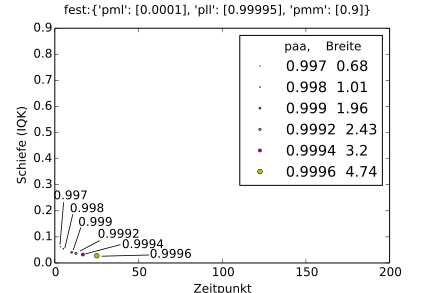
\includegraphics[width=\textwidth]{bilder/3fest_09_00001_p_099995.pdf}
\caption{$p_{mm}$ und $p_{ml}$ groß}
\end{subfigure}
\begin{subfigure}[t]{0.5\textwidth}
\includegraphics[width=\textwidth]{bilder/3fest_09_0001_p_099995}
\caption{$p_{mm}$ groß und $p_{ml}$ klein}
\end{subfigure}
\vspace*{7mm}
\begin{subfigure}[b]{0.5\textwidth}
\includegraphics[width=\textwidth]{bilder/3fest_01_00001_p_099995}
\caption{$p_{mm}$ klein und $p_{ml}$ groß}
\end{subfigure}
\begin{subfigure}[b]{0.5\textwidth}
\includegraphics[width=\textwidth]{bilder/3fest_01_0001_p_099995}
\caption{$p_{mm}$ und $p_{ml}$ klein}
\end{subfigure}
\caption{Der Einfluss von $p_{aa}$ auf die Peaks abhängig von $p_{mm}$ und $p_{ml}$}
\label{einfluss_paa}
\end{figure}

In Abbildung \ref{einfluss_paa} ist beispielhaft der Einfluss von Parameter $p_{aa}$ auf die Peaks gezeigt. Der Einfluss von $p_{aa}$ auf den Zeitpunkt wird mit steigendem $p_{mm}$ immer kleiner und reicht dadurch von minimalem Einfluss und recht frühen Peaks bei jeder Wahl von $p_{aa}$ bis zu sehr großem Einfluss und Peaks, die je nach $p_{aa}$ über das ganze Spektrum verteilt sind. Damit hat $p_{aa}$ einen ähnlichen Einfluss wie pmm. $p_{aa}$ hat nur dann einen relevanten Einfluss auf die Schiefe, wenn $p_{ml}$ groß ist. Der Einfluss auf die Breite ist mäßig und wird größer, wenn $p_{ml}$ und $p_{ll}$ klein sind.

Der Einfluss von $p_{ll}$ auf den Zeitpunkt ist minimal (Punkte liegen mehr oder weniger alle auf einer fast geraden nach oben)

\section{Laufzeiten}
